\documentclass[sn-aps]{sn-jnl}% Math and Physical Sciences Reference Style

\jyear{2021}%

\begin{document}

\title[Space Weather Effects on Critical Infrastructure]{Space Weather Effects on Critical Infrastructure}

%%=============================================================%%
%% Prefix	-> \pfx{Dr}
%% GivenName	-> \fnm{Joergen W.}
%% Particle	-> \spfx{van der} -> surname prefix
%% FamilyName	-> \sur{Ploeg}
%% Suffix	-> \sfx{IV}
%% NatureName	-> \tanm{Poet Laureate} -> Title after name
%% Degrees	-> \dgr{MSc, PhD}
%% \author*[1,2]{\pfx{Dr} \fnm{Joergen W.} \spfx{van der} \sur{Ploeg} \sfx{IV} \tanm{Poet Laureate} 
%%                 \dgr{MSc, PhD}}\email{iauthor@gmail.com}
%%=============================================================%%

\author*[1,2]{\fnm{G{\'a}bor} \sur{Facsk{\'o}}}\email{facsko.gabor@uni-milton.hu}

\author[2,3]{\fnm{Gergely} \sur{Kob{\'a}n}}\email{koban.gergely@wigner.hu}

\author[2,3]{\fnm{Nikolett} \sur{Bir{\'o}}}\email{biro.nikolett@wigner.hu}

\author[2,4]{\fnm{Munkhjargal} \sur{Lkhagvadorj}}\email{l.munkhjargal@wigner.hu}

\affil*[1]{\orgdiv{Department of Informatics}, \orgname{Milton Friedman University}, \orgaddress{\street{Kelta~utca~2.}, \city{Budapest}, \postcode{1039}, \state{Budapest}, \country{Hungary}}}

\affil[2]{\orgdiv{Department of Space Physics and Space Technology}, \orgname{Wigner Research Centre for Physics}, \orgaddress{\street{Konkoly-Thehe Miklos ut 29-33.}, \city{Budapest}, \postcode{1121}, \state{Budapest}, \country{Budapest}}}

\affil[3]{\orgdiv{Doctoral School of Physics}, \orgname{E{\"o}tv{\"o}s Lor{\'a}nd University}, \orgaddress{\street{P{\'a}zm{\'a}ny~P{\'e}ter~s{\'e}t{\'a}ny~1/A.}, \city{Budapest}, \postcode{1117}, \state{Budapest}, \country{Hungary}}}

\affil[4]{\orgdiv{Faculty of Science}, \orgname{E{\"o}tv{\"o}s Lor{\'a}nd University}, \orgaddress{\street{P{\'a}zm{\'a}ny P{\'e}ter s{\'e}t{\'a}ny 1/A}, \city{Budapest}, \postcode{1117}, \state{Budapest}, \country{Hungary}}}


%%==================================%%
%% sample for unstructured abstract %%
%%==================================%%

\abstract{Gas pipelines, transmission lines, overhead wires, transformers, GNSS navigation, and telecommunication systems are part of critical infrastructure. Industry, transportation, service operations, farming, and everyday life highly depend on this infrastructure. However, these systems are very sensitive to solar activity. Therefore, all activities above are vulnerable and defenseless against the catastrophic changes in Earth’s cosmic environment.
  
  The Solar System is dominated by the influence of our star. In the Solar System, all objects are bounded gravitationally and the Sun’s radiation provides the energy par example for the terrestrial biosphere. A small fraction of the energy produced in the core of our star turns into a magnetic field and emits the constant high-velocity plasma flow, the solar wind. Solar magnetic activity produces radiation and ejects matter from the upper atmosphere of our star. The magnetic field frozen to the solar wind plasma interacts with the planetary magnetic fields and atmospheres. These phenomena, called Space Weather have a serious influence on the radiation environment of Earth where telecommunication, GNSS, meteorological, and other purpose satellites are located. The conductivity and transparency of the higher partly ionized atmospheric layer, the ionosphere also depend on solar radiation and activity. This fact makes the navigation and communication systems dependent on solar activity. Finally, the solar magnetic activity creates magnetic variations in the terrestrial magnetic field and induces currents in gas pipelines, transmission lines, overhead wires, and transformers.
  
In this short briefing, we introduce the solar activity phenomena, and their influence on our planet’s cosmic neighborhood and provide a detailed description of the Space Weather effects on critical infrastructure. Finally, we share and detail some methods to forecast the critical Space Weather effects and protect the infrastructure mentioned previously.}

\keywords{Space Weather, Solar Activity, Geomagnetically Induced Currents, Telecommunication, Global Navigation Satellite System disturbances}

\maketitle

\section{Introduction}
\label{sec:intro}

This paper is supposed to be a brief review of the cosmic phenomena that endangers our planet and civilization on planet Earth. 

\subsection{Definitions and clarifications}
\label{sec:def}

Here, the critical infrastructure (CI) means submarine internet cables, gas pipelines, transmission lines, overhead wires, transformers, Global Navigation Satellite System (GNSS) navigation, satellite telecommunication, and HF radio telecommunication systems. Submarine internet cables, gas pipelines, transmission lines, overhead wires, and transformers are long, conductive objects therefore they are sensitive to quickly varied magnetic fields. GNSS navigation, satellite telecommunication, and HF radio telecommunication systems depend on the transmission and reflection ability of the ionosphere (that is a conductive layer of the upper atmosphere at $\sim$120\,km altitude).

The Space Weather (SW) term has two meanings. It is a new(er) name for the research of the solar-terrestrial relationship. Additionally, the expression covers the efforts to predict the conditions of the near-Earth cosmic environment, the ionosphere, and the surface of our planet \cite{scherer05:_space_weath}. 


\subsection{Introduction to space weather}
\label{sec:swintro}

The main drive of the space weathe in the Solar System is the Sun. All planets, moons and other objects are located in its extended and expanding atmosphere, the solar wind. The solar wind interacts with the magnetic field of our star.

\subsubsection{The magnetic activity of our star}
\label{sec:magnact}

We have an aggressive and dominant neighbor: the Sun (Fig.~\ref{fig:sunvisible}). During total solar eclipes the solar corona, this hot, extended and relatively faint part of the atmosphere of our star becomes visible. You can see filaments in the corona and its shape and extension varies depending the Sun's magnetic activity (Fig.~\ref{fig:sunvisible}, top left). In visible light you can see sunspot on the disc of the Sun (Fig.~\ref{fig:sunvisible}, top right). These regions have lower temperature than their neigbourhood therefore they look darker (Fig.~\ref{fig:sunspot}). In the wavelength of $H_{\alpha}$ (656.28\,nm) the granulation, the continious boiling motion of the solar plasma is visible (Fig.~\ref{fig:sunvisible}, bottom). The energy produced in the solar interour leaves our star by conductivity in it outmost layer. This conductive motion of the conductive solar plasma and the rotation of the Sun set up and moves the solar dynamo that produces strongmagnetic field. The magnetivity of our star dominates the space nearly the Sun. This region of the space is called heliosphere \cite{stix04:_sun_introd}. The magnetic activity of the Sun makes serious disturbances in the navigation and the communication \cite{scherer05:_space_weath}. 

Our star produces energy by termonuclear fusion in its core. The produced energy flows our by radiation until $\sim$70\,\% of its radious. There the material of the Sun become convective. The energy is transported by moving material. The Sun rotates quite quickly. The material of our star is in so-called plasma state: its atoms lost their electrons and build up a quasi-neutral, highly conductive material. The convective and rotational motions of the highly conductive material set up a dynamo. Therefore the Sun has a very strong magnetic field. The magnitude of this magnetic field is 1\,Tesla (T). The magnitude of Earth's magnetic field is from 25000\,nT to 65000\,nT. In Magnetic Resonance Imaging instrument the strength of the magnetic field is $\sim$1\,T in a 0.5\,m$\times$0.5\,m$\times$0.5\,m cube. On the Sun the diameter of the magnetic flux tubes are 12000\,km (2\,$R_{Earth}$) and their length could be a few hundred tousand\,km. Those solar magnetic structures consist of vast amount of energy. It is only $\sim$1\,\% of the energy produced by the fusion in the solar core. However, the magnetic filed and the magnetic activity of the Sun has a dominant influence on the nearby space around the Sun, to the heliosphere \cite{scherer05:_space_weath,stix04:_sun_introd}.

\subsubsection{Flares and coronal mass ejections}
\label{sec:cme}

Sometimes two solar flux tubes with opposite direction situated close to each other and gradually forms an ``X'' shape configuration (Fig.~\ref{fig:reconnection}). If these flux tubes are enough close to each other it becomes energetically better configuraton if half-half of the opposite tubes form a shorter bended structure (Fig.~\ref{fig:reconnection}). Its phenomena is called reconnection and bursts huge amount of energy. This region of the solar atmosphere reaches 15-20\,million\,K degree. (The temperature of the arbitrary solar surface is 6000\,K and the solar core where the termonuclear fusion produces the energy is only 16\,million\,K degree.) A bright flash in vissible light, X-ray and radio bursts are ejected. Charged particles are accelerated to high energy. A jet is ejected to the solar surface and usually (but not always) a huge amount of hot plasma launched to the heliosphere. Its name is coronal mass ejection (CME) or solar storm (Fig.~\ref{fig:cme}). The ejected plasma node remains connected magnetically to the Sun during its travel in the Solar System (Fig.~\ref{fig:cme}, bottom). CMEs can also occur independently. A large CME could contain a billion tons of plasma that can be accelerated to several thousand km per seconds. Solar material flies through the interplanetary medium, impacting any planet (Fig.~\ref{fig:cmeearth}) or spacecraft in its path \cite{scherer05:_space_weath,stix04:_sun_introd}.

\subsubsection{The solar wind and solar wind streams}
\label{sec:sw}

The reason of all troubles in the heliosphere is the atmosphere of the Sun (Fig.~\ref{fig:corona}, top left). The temperature of the photosphere is 6000\,K. The temperature of the chromosphere which is above the photosphere is around 10000\,K. Finally, the temperature of the corona which exists above the chromosphere is around 1000000\,K. You can see that in the solar atmosphere, the outer layers have higher temperatures (Fig.~\ref{fig:corona}, top left). A strong, fast plasma flow originates from the outer layer of the solar corona, the solar wind (Fig.~\ref{fig:cmeearth}). The distribution of the solar wind speed has two maxima at 400\,km/s and 800\,km/s \cite{mccomas98:_ulyss}. These type of solar wind are called slow and fast solar wind or slow and fast solar wind streams. The slow solar wind is originated from the normal solar coronal. In X$-$ray and extreme ultraviolet (EUV) observations the solar corona has larger regions so-called coronal holes that look dark in these wavelengths (Fig.~\ref{fig:corona}, top right). The fast solar wind is ejected from these coronal holes \cite{scherer05:_space_weath,stix04:_sun_introd}. A magnetic field lines moves together with the solar wind plasma. You can say the magnetic field lines are frozen in the solar wind plasma. The solar wind moves radialy outward and the Sun rotates. Very soon, the angular speed of the plasma will be less than the angular speed of the solar rotation. Therefore, a spiral form of the magnetic field is created by these movements. Its name is Parker-spiral. The fast and slow solar wind streams interact to each other and forms compressional and rarefraction regions (Fig.~\ref{fig:corona}, bottom). These regions (co$-$called corotating interaction regions, CIRs) could hits the terrestrial magnetosphere \cite{scherer05:_space_weath}. Their effects and disturbances are not as strong as the effects of a CME however it could cause serious problems for the critical insfrastructure. 

\subsubsection{The terrestrial magnetosphere and the aurora}
\label{sec:magn}

\textbf{Slide~7} The solar wind enters to the terrestrial magnetosphere and creates aurora, magnetic disturbances, GICs and the radiation belts.

\section{Space Weather effects on critical infrastructure}
\label{sec:sweci}

The sources of the radiation: Cosmic rays. Solar Energetic Particles (SEP). Solar Flare Radiation. Solar Flare Radio Burst. Energetic Particle Belt Particles.

Damages and disturbances: Navigation errors. Signal scintillation. Disturbed reception. HF radio wave disturbances. Induced geoelectric field and current. Geomagentically induced currents in power. systems, submarine cables, gaspipelines and overhead wires.

Aurora: Important indicator of the activity. Beautiful tourist attraction.

Various nowcast and prediction systems: ESA, NASA, NOAA, CIRES, UK MET Office, PECASUS, Auroras Now!

\section{Summary}
\label{sec:sum}

The Sun dominates its neighborhood -> The heliosphere is the region dominated by the Sun. The solar wind comes from the solar corona. It interacts with the objects in the heliosphere. The energy produced by fusion flows outward and creates magnetic activity. The magnetic field creates solar spots, protuberances, filaments, and flares. The magnetic reconnections produce an incredible amount of energy. In this flash, the flare ejects particles into interplanetary space and the solar atmosphere. The flash could reach 20 MK and launch a coronal mass ejection (CME). The CMEs are material ejections to the interplanetary space. Their size could be much larger than the diameter of the Sun. If the CMEs reach the Earth they could create magnetic disturbances, aurora, and geomagnetically induced currents in the pipelines. They may ruin the communication equipment and electronic devices in the orbit of the Earth. These events cut short-wave communication by changing the conductivity of the ionosphere however they can disturb satellite communication and navigation systems.

The aurora is the consequence of the phenomena above. The aurora activity is permanent under the aurora oval. The intensity of the aurora is proportional to the bandwidth of the radio communication through the ionosphere. These events can be predicted and the critical infrastructure can be prepared. The satellite systems can be switched off
before the solar storm arrives.

The space weather is the events described above and their prediction. It has a direct application. The USA, China, Brazil, South Africa, Sweden, the UK, and the ESA have space weather forecast centres.

\backmatter

\bmhead{Acknowledgments}

This work was partially financed by the National Research, Development, and Innovation Office (NKFIH) FK128548 grant.

% -------------------------------------------------------------------------------------------------------------

\pagebreak

%\bibliographystyle{sn-chicago}
\bibliography{facsko_iccecip2022}

% -------------------------------------------------------------------------------------------------------------

\pagebreak

\begin{figure}[h]
\centering
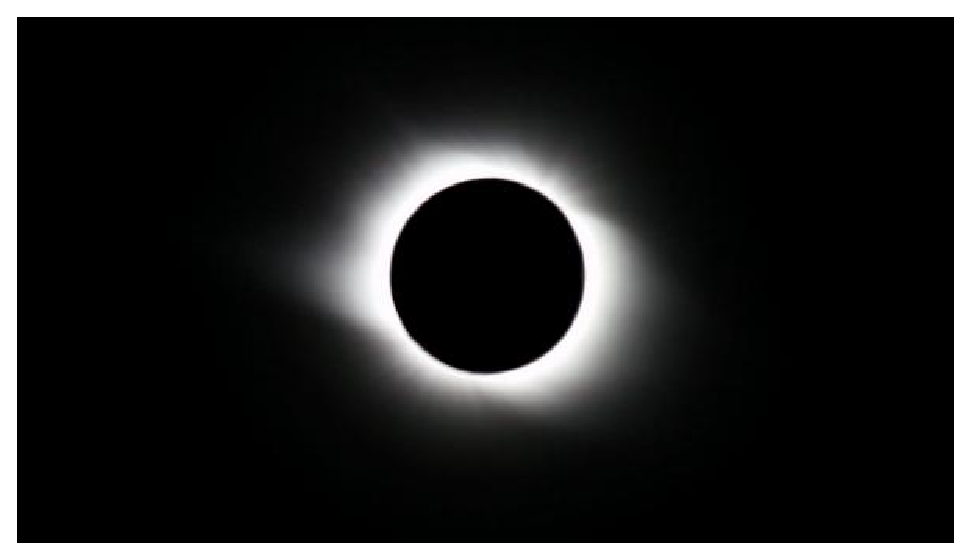
\includegraphics[width=0.51\textwidth]{facsko_iccecip2022-f01a.eps}
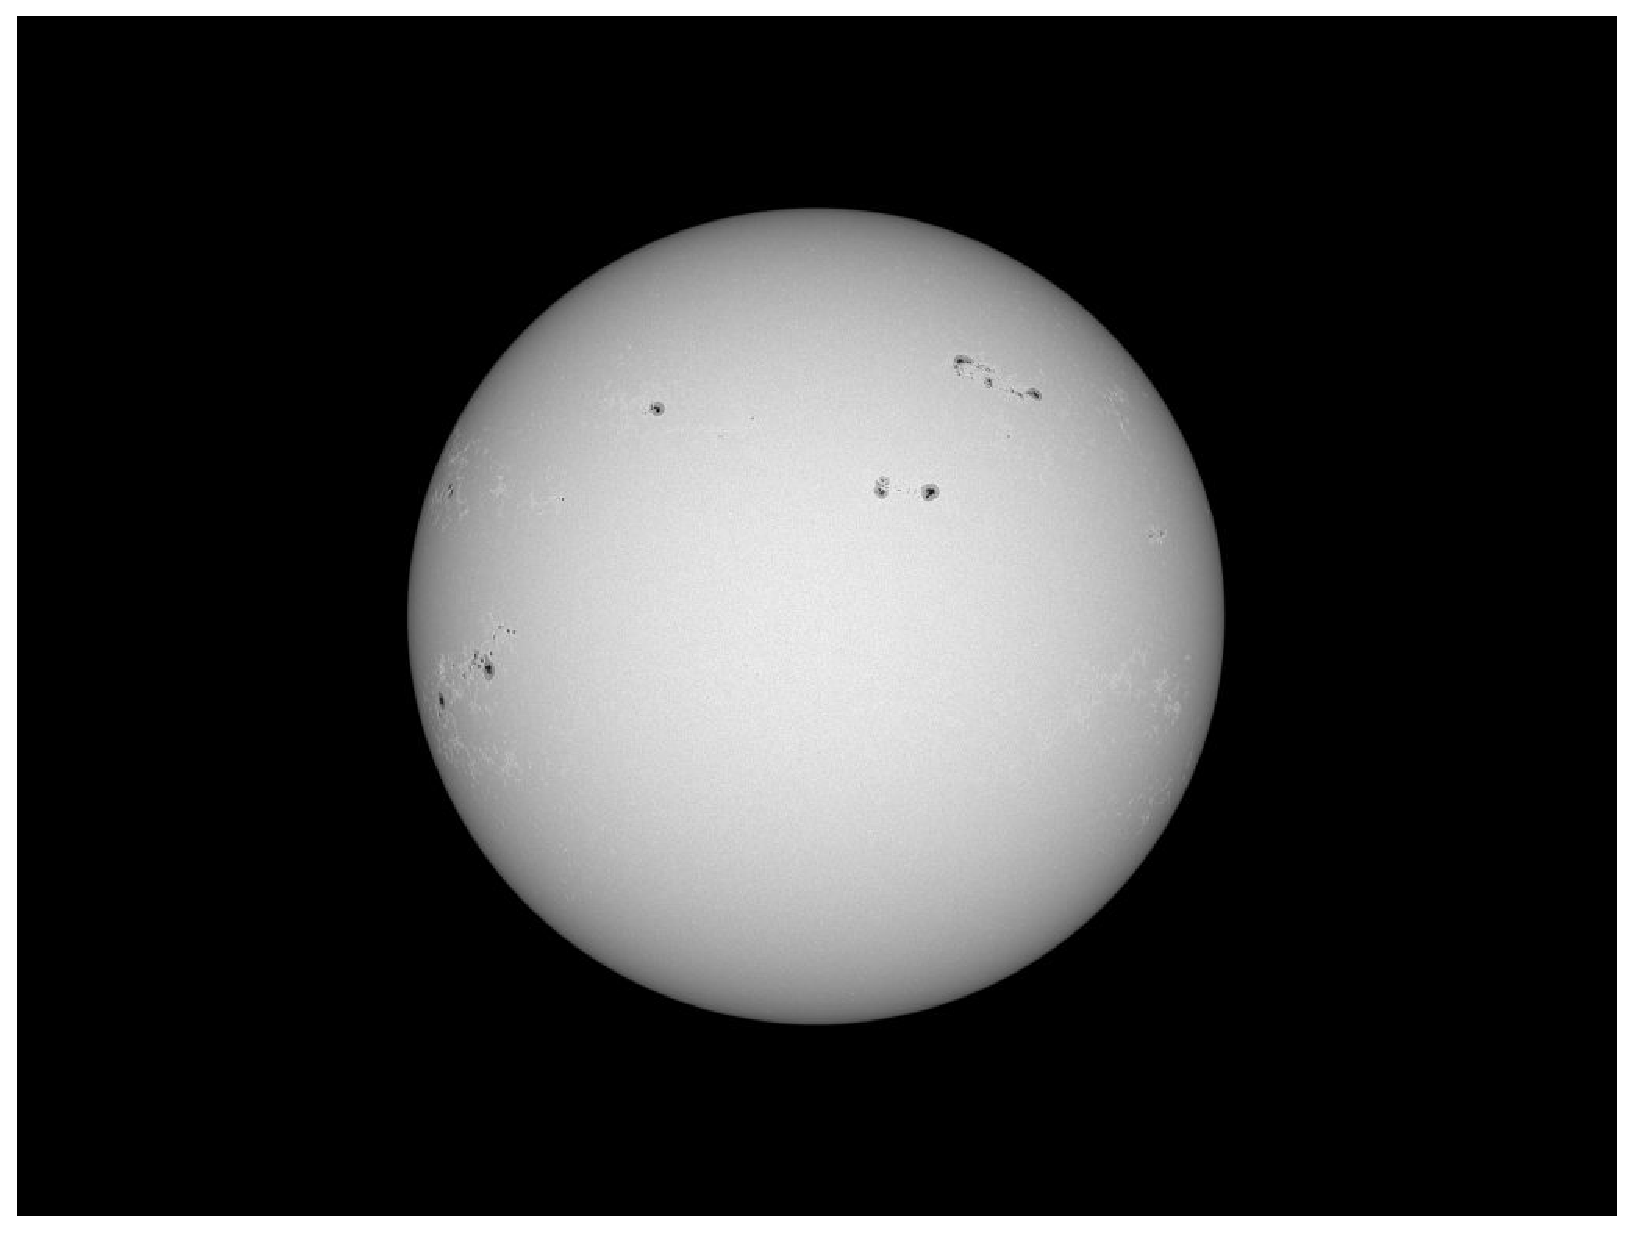
\includegraphics[width=0.38\textwidth]{facsko_iccecip2022-f01b.eps}
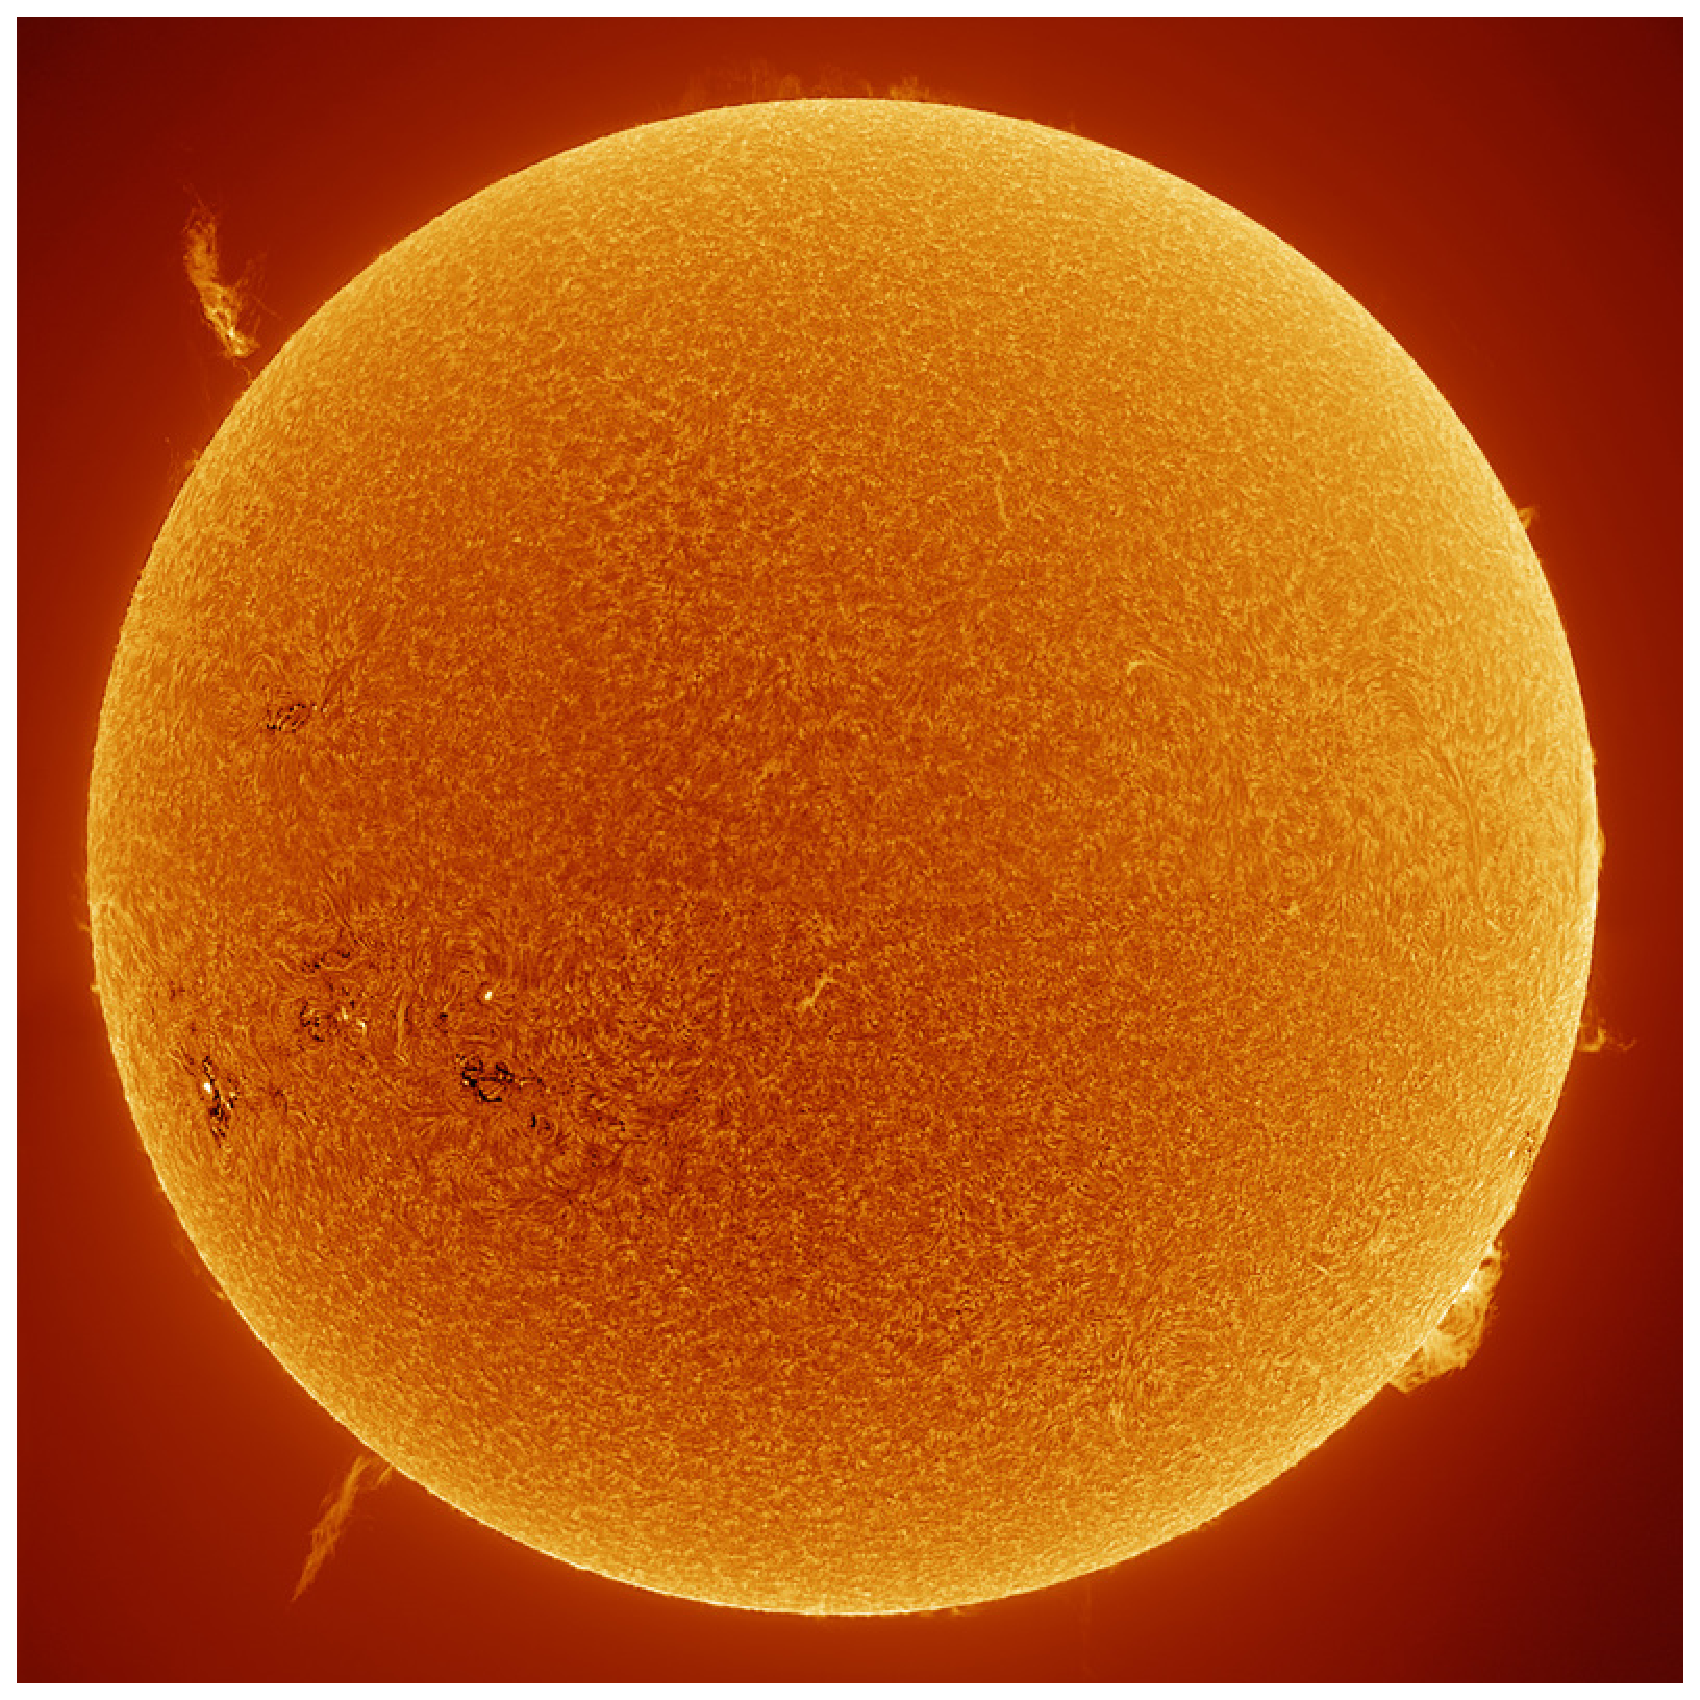
\includegraphics[width=0.9\textwidth]{facsko_iccecip2022-f01c.eps}
\caption{(Top left) During a total solar eclipse, the hot, relatively faint, extended upper atmosphere of the Sun (the solar corona) becomes visible. (Top right) Even in visible light, you can see structures, and spots on our star. (Bottom) Using $H_{\alpha}$ filter (656.28\,nm) the granulation of our stars becomes visible on the bottom of its transparent atmosphere (the so-called photosphere), and the protuberances, erupt structures around the disc as well. (Credit: https://www.timeanddate.com/, \url{https://c.tadst.com/gfx/600x337/total-solar-eclipse.jpg}; https://csillagtura.ro~\url{https://csillagtura.ro/wp-content/uploads/2023/02/20230213_T110800Z_timeisavgof3_s7c_nap_sun_solar_continuum_7p5nm_slc_AS_F500_lapl5_ap635_reg1_ps3.jpg}; Peter Borovszky \url{https://tavcso.hu/contents/img/gallery/1002555.jpg}.)}\label{fig:sunvisible}
\end{figure}


\begin{figure}[h]
\centering
\includegraphics[width=0.9\textwidth]{facsko_iccecip2022-f02.eps}
\caption{The sunspots are the prove of the magnetic activity of the Sun. The magnetic field lines intersect the photosphere and cool down a region. The colder regions look darker on the bright disc. (Credit: Encyclopedia Britannica, \url{https://cdn.britannica.com/12/96912-050-D5DB526D/group-region-Sunspot-Swedish-Solar-Telescope-image.jpg})}\label{fig:sunspot}
\end{figure}


\begin{figure}[h]
\centering
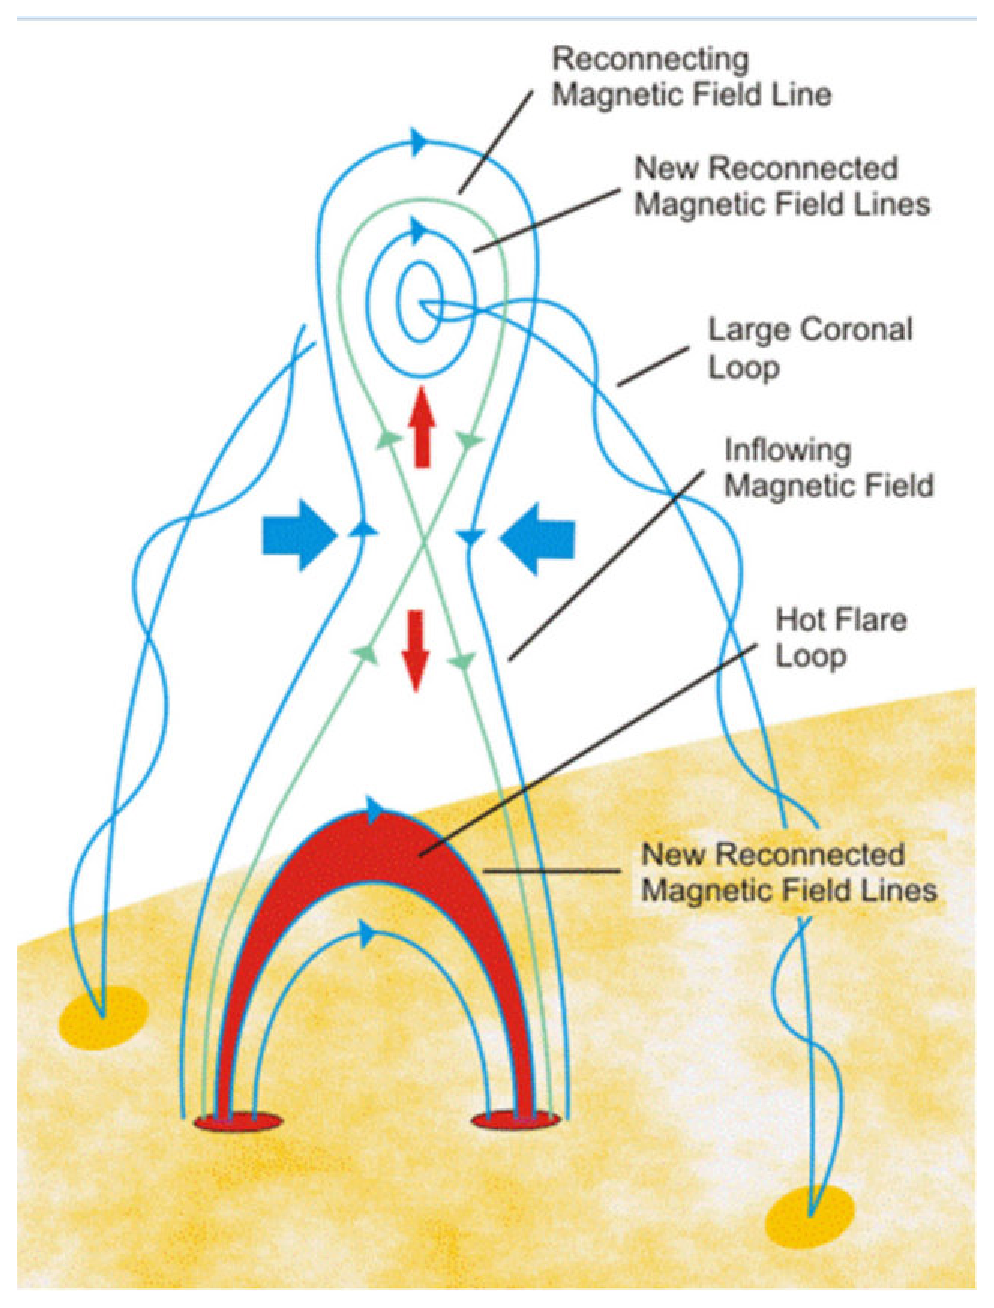
\includegraphics[width=0.9\textwidth]{facsko_iccecip2022-f03.eps}
\caption{A draft of magnetic reconnection and a solar flare. (Credit: Gordon Holman and NASA, \url{https://www.researchgate.net/profile/Jose-Campos-Rozo/publication/318404921/figure/fig11/AS:631675696451597@1527614630141/2-An-illustrated-model-of-magnetic-reconnection-and-solar-flare-diagram-Image-Credit_W640.jpg})}\label{fig:reconnection}
\end{figure}

\begin{figure}[h]
\centering
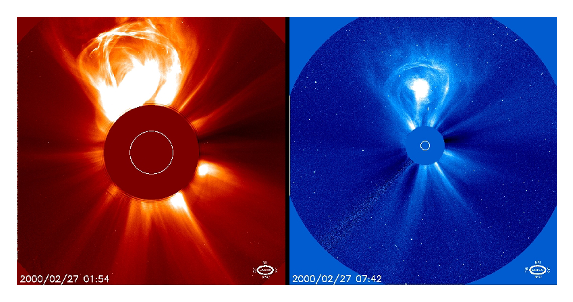
\includegraphics[width=0.9\textwidth]{facsko_iccecip2022-f04a.eps}
\includegraphics[width=0.9\textwidth]{facsko_iccecip2022-f04b.eps}
\caption{(Top left and right) A coronal mass ejection on February 27, 2000 taken by SOlar and Heliopsheric Observatory (SOHO) Large Angle and Spectrometric Coronagraph Experiment (LASCO) C2 and C3. A CME blasts into space a billion tons of particles traveling millions of miles an hour \cite{brueckner95:_large_angle_spect_coron_lasco,domingo95:_soho}. (Bottom) Solar Dynamic Observatory (SDO) image of the Earth to scale with the filament eruption on August 31, 2012 \cite{pesnell12:_solar_dynam_obser_sdo}. (Credit: SOHO ESA \& NASA, \url{https://www.nasa.gov/sites/default/files/thumbnails/image/faq4.jpg}; NASA Goddard Space Flight Center, \url{https://svs.gsfc.nasa.gov/vis/a010000/a011000/a011095/earth\_scale.jpg})}\label{fig:cme}
\end{figure}

\begin{figure}[h]
\centering
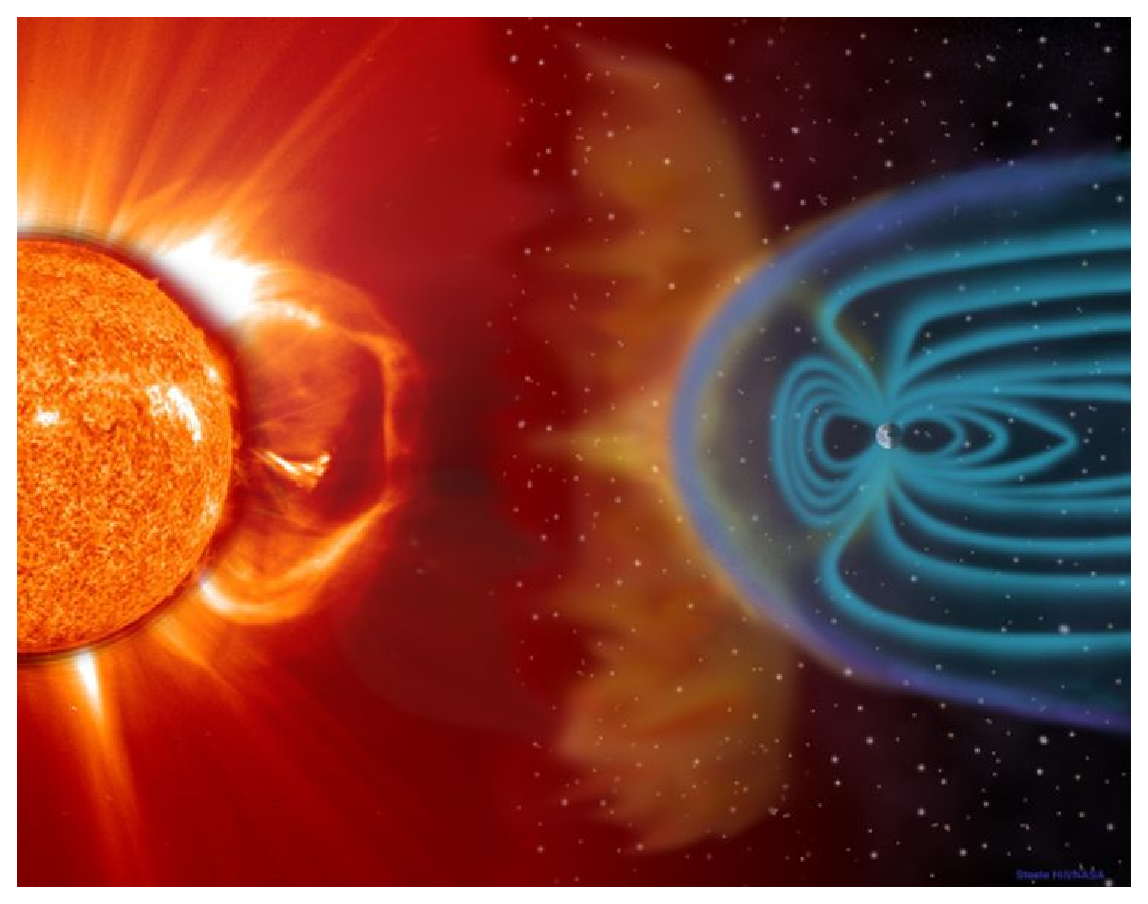
\includegraphics[width=0.9\textwidth]{facsko_iccecip2022-f05.eps}
\caption{The CMEs could reach our planet. The Earth's magnetic field, displayed in blue, protects our planet from the harmful radiations of our star. CMEs causes the colorful auroras around the poles as they interact with Earth's magnetic shield and can disrupt GPS and communication satellites. (Credit: NASA Goddard Space Flight Center, \url{https://res.cloudinary.com/dtpgi0zck/image/upload/s--eqSnFkH6--/c_fit,h_580,w_860/v1/EducationHub/photos/solar-wind.jpg})}\label{fig:cmeearth}
\end{figure}

\begin{figure}[h]
\centering
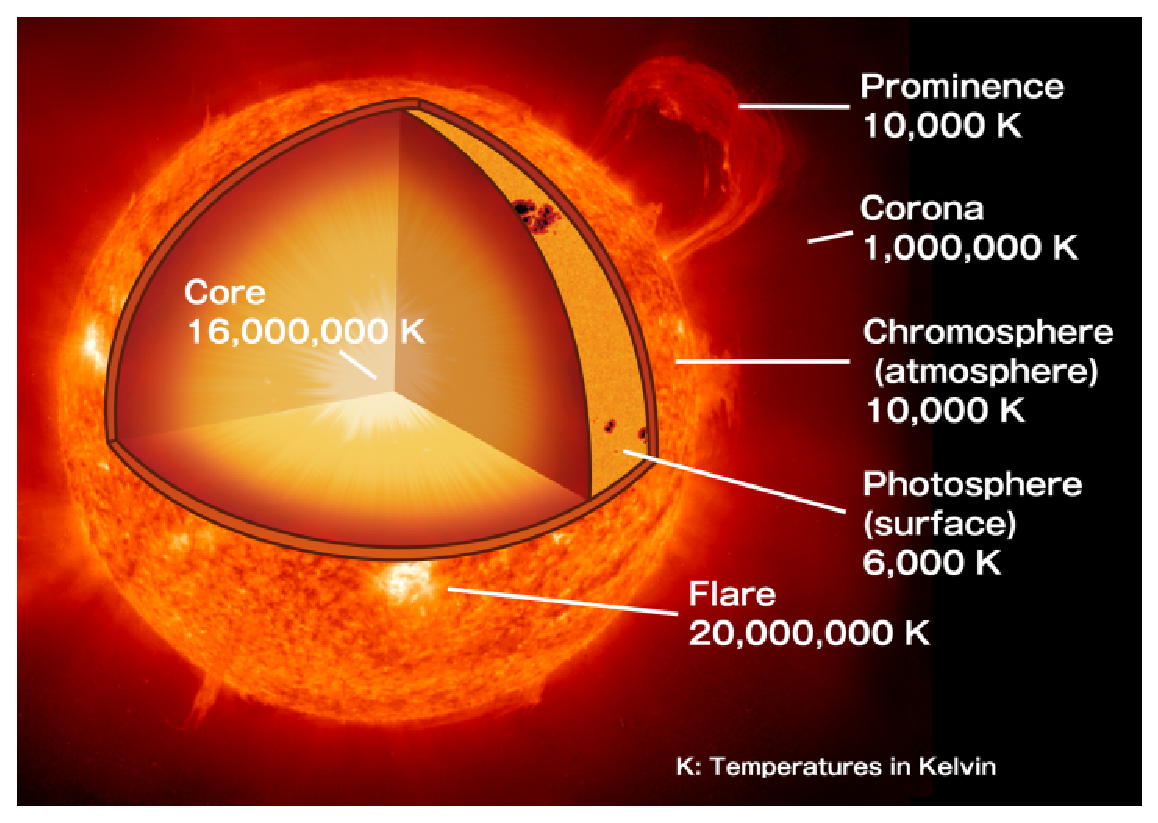
\includegraphics[width=0.525\textwidth]{facsko_iccecip2022-f06a.eps}
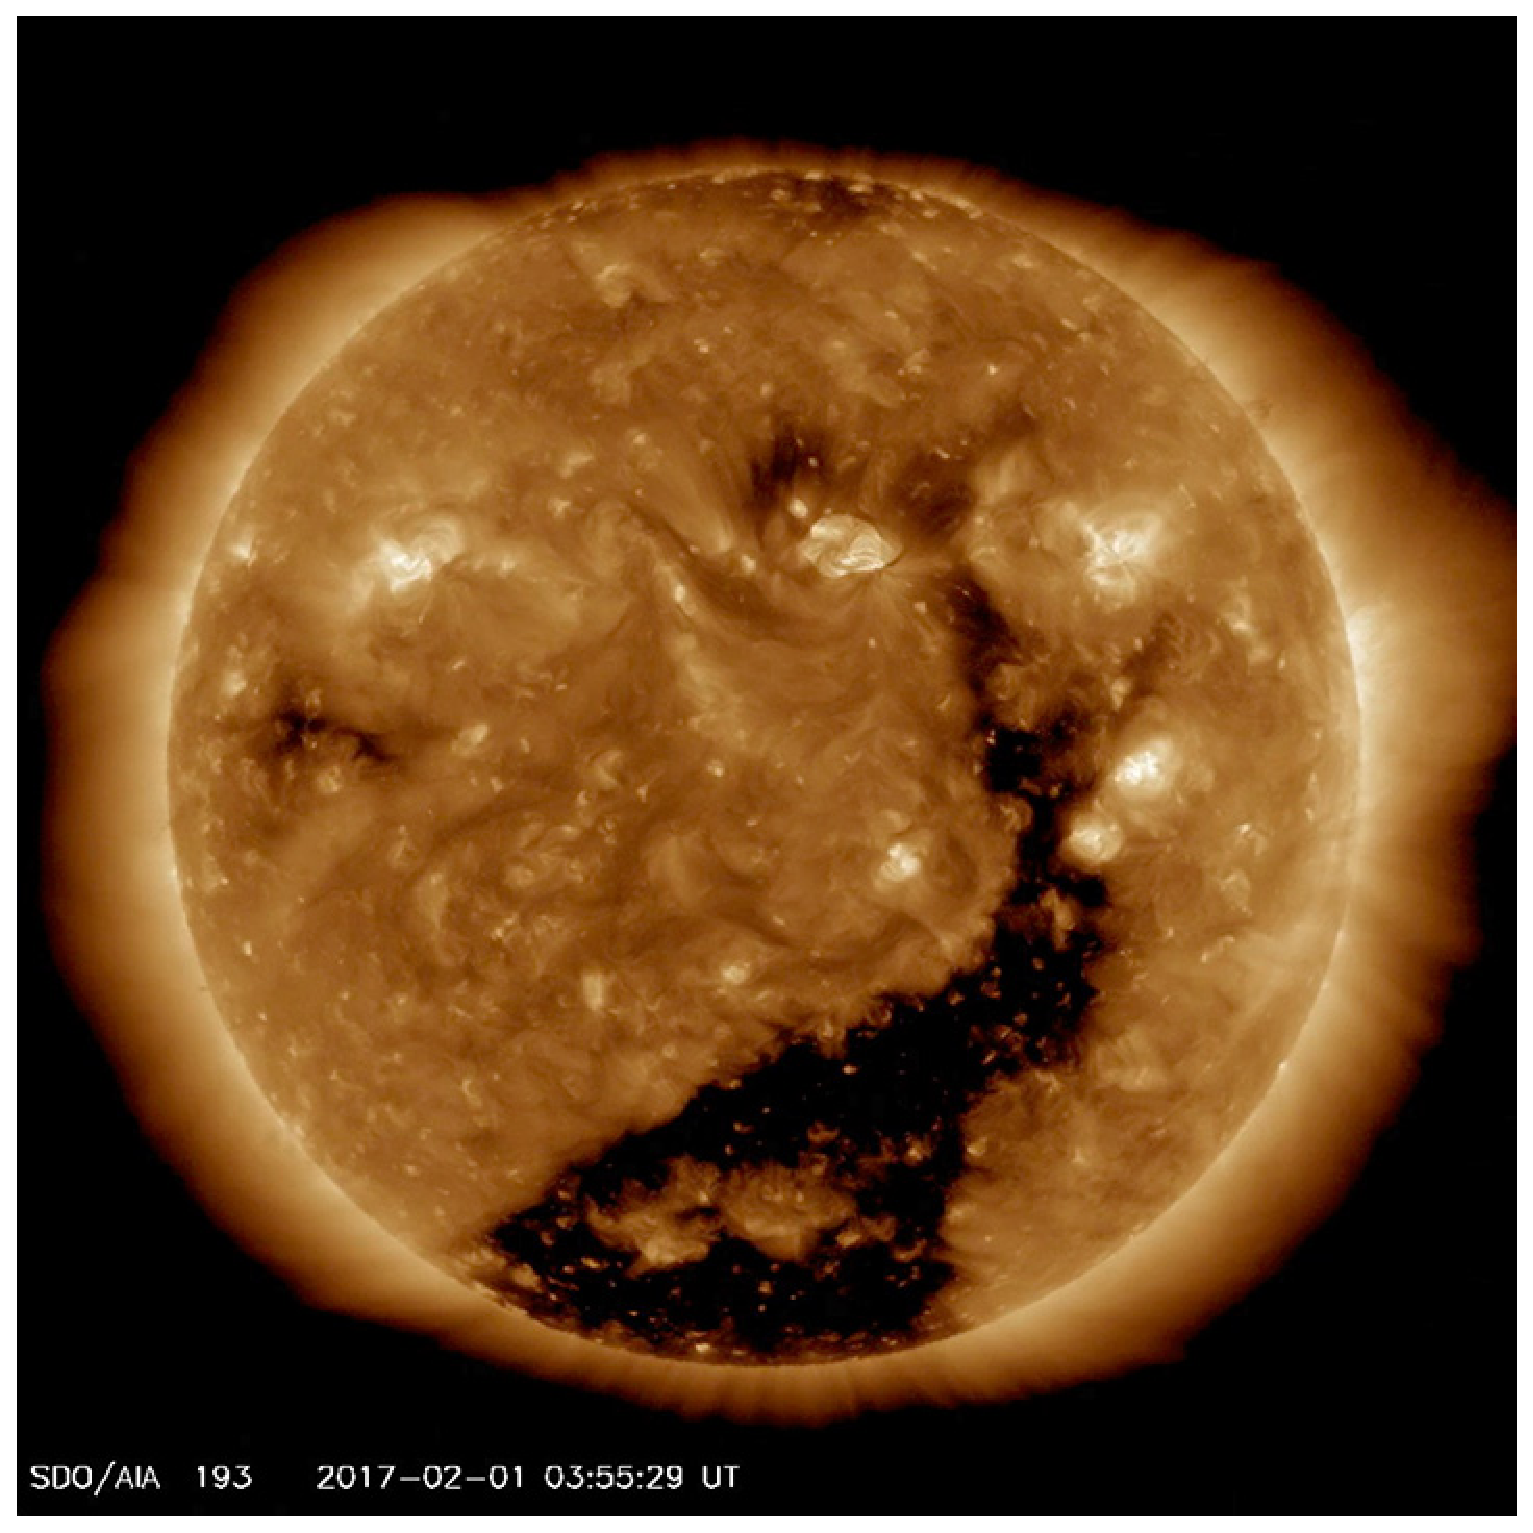
\includegraphics[width=0.37\textwidth]{facsko_iccecip2022-f06b.eps}
\includegraphics[width=0.9\textwidth]{facsko_iccecip2022-f06c.eps}
\caption{(Top left) The structure and temperature of the solar atmosphere. The temperature of the solar corona is much higher than the inner layers of the solar atmosphere. A strong plasma flow, the solar wind originates from the outer layers of the solar corona. (Top right) A coronal hole observation in extreme ultraviolet light of the SDO / Atmospheric Imaging Assembly (AIA) on February 1, 2017 \cite{pesnell12:_solar_dynam_obser_sdo,lemen12:_atmos_imagin_assem_aia_solar}.  Coronal holes are areas of open magnetic field from which solar wind particles stream into space. (Bottom) The solar wind structure in the ecliptic plane showing the fast (slow) solar wind in red (blue). A magnetic field lines moves together with (or frozen in) the solar wind plasma. The plasma moves radialy outward and the Sun rotates. These movements creates a spiral form of the magnetic field, the so-called Parker-spiral. The streams interact to each other and forms compressional and rarefraction regions. These regions (so-called corotating interaction regions, CIRs) hits the terrestrial magnetosphere. (Credit: Institute of Space and Astronautical Science (ISAS) / Japan Aerospace Exploration Agency (JAXA), \url{https://hinode.nao.ac.jp/assets_c/2017/02/41406e85f7de7aadb1d61876ea3b7b03aa22a9c6-thumb-720xauto-2671.png}; SDO/AIA, NASA, \url{https://sdo.gsfc.nasa.gov/assets/gallery/preview/Coronal_hole_193_Feb.jpg}; \cite{zhang21:_earth}, Fig.~30, \url{https://media.springernature.com/full/springer-static/image/art\%3A10.1186\%2Fs40645-021-00426-7/MediaObjects/40645\_2021\_426\_Fig30\_HTML.png})}\label{fig:corona}
\end{figure}


%\begin{figure}[h]
%\centering
%\includegraphics[width=0.9\textwidth]{facsko_iccecip2022-f07.eps}
%\caption{A coronal hole observation in extreme ultraviolet light of the SDO / Atmospheric Imaging Assembly (AIA) on February 1, 2017 \cite{pesnell12:_solar_dynam_obser_sdo,lemen12:_atmos_imagin_assem_aia_solar}.  Coronal holes are areas of open magnetic field from which solar wind particles stream into space.  (Credit: SDO/AIA, NASA, \url{https://sdo.gsfc.nasa.gov/assets/gallery/preview/Coronal_hole_193_Feb.jpg})}\label{fig:choles}
%\end{figure}


%\begin{figure}[h]
%\centering
%\includegraphics[width=0.9\textwidth]{facsko_iccecip2022-f08.eps}
%\caption{The solar wind structure in the ecliptic plane showing the fast (slow) solar wind in red (blue). A magnetic field lines moves together with (or frozen in) the solar wind plasma. The plasma moves radialy outward and the Sun rotates. These movements creates a spiral form of the magnetic field, the so-called Parker-spiral. The streams interact to each other and forms compressional and rarefraction regions. These regions (so-called corotating interaction regions, CIRs) hits the terrestrial magnetosphere. (Credit: \cite{zhang21:_earth}, Fig.~30, \url{https://media.springernature.com/full/springer-static/image/art\%3A10.1186\%2Fs40645-021-00426-7/MediaObjects/40645\_2021\_426\_Fig30\_HTML.png})}\label{fig:streams}
%\end{figure}




\end{document}
